\chapter{Popis implementace}
% TODO:
% implementace
%     - popsat hierarchii
%     - dole jsou nejaky ECS implementace
%     - nad nimi abstrakcni vrstva
%     - s tou pracuje hra
%     - ta je pak nejak slozena
%     - takhle az k detailum
V této kapitole si představíme klíčové a zajímavé části implementace naší hry. Pro více detailů o implementaci je možné nahlédnout do kódu, který obsahuje dokumentační komentáře.

Pro celý projekt používáme jedno C\# řešení. To obsahuje dva C\# projekty. Prvním je hra a druhým je měření, které používá vytvořenou hru pro měření výkonu ECS knihoven. V této kapitole se budeme věnovat pouze hře a na měření se zaměříme později.

Projekt hry se skládá ze tří částí. První částí jsou implementace ECS knihoven, které implementují abstrakční vrstvu. Nad nimi je samotná abstrakční vrstva, která je druhou částí. Třetí část je hra samotná, která namísto konkrétní ECS knihovny používá abstrakční vrstvu.

\section{Abstrakční vrstva}
\label{sec:abstract-layer}
Abstrakční vrstva se nachází ve jmenném prostoru \texttt{WorldSimulator.ECS.AbstractECS}. Ve jmeném prostoru \texttt{WorldSimulator.ECS} krom abstrakční vrstvy lze také nalézt jednotlivé její implementace.

\subsection{Systémy}
V ECS jsou systémy zodpovědné za iterace a zpracování entit. Jelikož každá ECS knihovna iteruje přes entity jiným způsobem, a zároveň chceme definovat zpracování entit (herní logiku) pouze jednou, bude nutné implementaci rozdělit do několika tříd. Vztah tříd, které souvisejí se systémy je možné vidět na obrázku~\ref{fig:abstract-layer-systems}.

\begin{figure}[!htb]
  \centering
  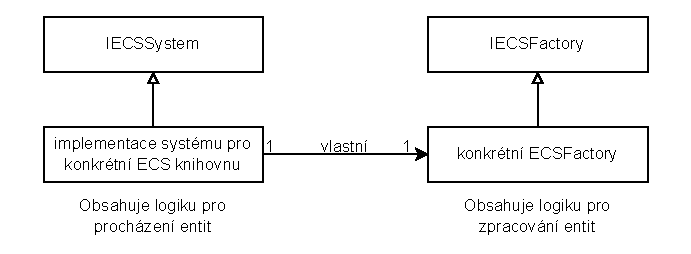
\includegraphics[width=0.66\linewidth]{img/abstract-layer-systems.pdf}
  \caption{Vzah tříd souvisejících se systémy.}
  \label{fig:abstract-layer-systems}
\end{figure}

\texttt{IECSSystem} je rozhraní ze kterého dědí každý systém, každá ECS knihovna poté poskytne svojí implementaci systému. Tyto implementace obsahují pouze logiku pro iteraci neboli procházení přes jednotlivé entity. Každá implementace systému bude vlastnit konkrétní \texttt{ECSFactory} dědicí od \texttt{IECSFactory}. Jednotlivé \texttt{ECSFactory} jsou zodpovědné za zpracování entit. Jednotlivé implementace rozhraní \texttt{IECSSystem} jsou generické typy, které přijímají typ entity procesoru a také typy komponent, které od entit vyžadují jako generické parametry.

Jako příklad si uvedeme třídu \texttt{ArchSystem<TEntityProcessor, TComponent>}. Jedná se o implementaci systému. Tento systém obsahuje logiku pro iteraci entit z ECS knihovny \textit{Arch}~\cite{Arch}. Příkladem konkrétního \texttt{EntityProcessor} je například třída \texttt{MovementSystem}, která řeší zpracování entit s komponentami \texttt{Position} a \texttt{Movement} a obsahuje logiku zodpovědnou za jejich pohyb.

Z pohledu hry jednotlivé implementace \textit{EntityProcessor} představují samotné systémy, jelikož hra nekouká na to jak jsou entity iterovány a zajímá je jenom samotná herní logika. Proto se kód, který pracuje s hrou odkazuje na \texttt{EntityProcessor} jako na systém. Ovšem z pohledu abstrakční vrstvy je nutné rozlišovat \texttt{System} jako typ, který obsahuje logiku pro iteraci entit a \texttt{EntityProcessor} jako typ, který obsahuje logiku pro zpracování entit. Autor si je vědom, že tyto pohledy mohou vést k matoucí terminologii, ovšem v kódu jsou již používány na příliš mnoho místech.

\subsection{ECSFactory}
\texttt{ECSFactory} je abstraktní třída. Typy, které z ní dědí jsou zodpovědné za tvorbu instancí související s abstrakční vrstvou. Vztah typů souvisejících s \texttt{ECSFactory} je možné vidět na obrázku~\ref{fig:abstract-layer-ecsfactory}.

\begin{figure}[!htb]
  \centering
  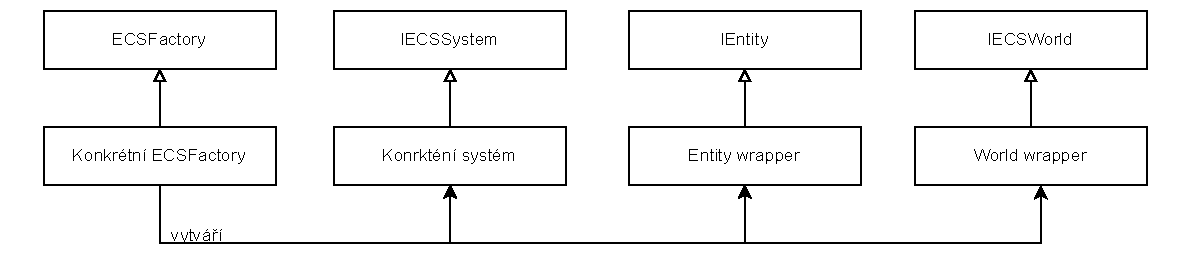
\includegraphics[width=1.0\linewidth]{img/abstract-layer-ecsfactory.pdf}
  \caption{Vzah tříd souvisejících s \texttt{ECSFactory}.}
  \label{fig:abstract-layer-ecsfactory}
\end{figure}

Typ, který dědí od \texttt{ECSFactory} musí implementovat metody pro vyváření instancí wrapperu entity a wrapperu \textit{worldu}. Skrze konstruktor svému předku také předá typy jednotlivých systémů (tříd dědicích od \texttt{IECSSystem}). Wrapper entity je třída dědicí od rozhraní \texttt{IEntity} a je zodpovědná za přidávání a odebíraní komponent na dané entitě. Wrapper \textit{worldu} je třída dědicí od rozhraní \texttt{IECSWorld}. Tento wrapper implementuje metodu \texttt{Update}, která je zodpovědná za aktulizaci stavu \textit{worldu}.

\section{Hra}
Celá hra je reprezentována třídou \texttt{Game}, té je skrze konstruktor předána konkrétní instance \texttt{ECSFactory}. Jednotlivé instance \texttt{ECSFactory} reprezentují jednotlivé ECS knihovny a volba této instance představuje volbu ECS knihovny se kterou bude hra pracovat.

První herní stav je hře předán skrze metodu \texttt{SwitchState}. Samotná hra je spuštěna metodou \texttt{Run}.

\subsection{Herní stavy}
Celá hra se může skládat z několika herních stavů. Každý herní stav je reprezentován třídou dědicí od \texttt{GameState} a představuje herní obrazovku. Například hra může mít herní stavy \texttt{MenuState}, reprezentující obrazovku s hlavním menu, \texttt{LevelState}, reprezentující obrazovku s úrovní hry a \texttt{GameOverState}, reprezentující obrazovku konce hry.

V jeden moment může být aktivní pouze jeden herní stav, ten lze zvolit za pomoci metody \texttt{SwitchState} na třídě \texttt{Game}.

Každý herní stav obsahuje svoji instanci \texttt{ECSWorld}, která reprezentuje \textit{world} herního stavu, \texttt{Camera}, která reprezentuje herní kameru herního stavu a \texttt{UILayer}, která spravuje prvky uživatelského rozhraní herního stavu.

Každý herní stav vlastní svoje systémy. Ty se rozdělují na klasické systémy a systémy, které pracují s logikou vykreslování.

Konkrétní herní stavy (instance tříd dědicích od \texttt{GameState}) jsou zodpovědné za vytváření entit, systémů a prvků uživatelského rozhraní.

I přesto, že hra momentálně obsahuje pouze jeden herní stav (konkrétně \texttt{LevelState}), tak by bylo snadné ji rozšířit o další herní stavy jako je například obrazovka s hlavním menu.

\texttt{LevelState} reprezentuje herní obrazovku obsahující samotný gameplay. Váže se k ní třída \texttt{LevelFactory}, která obsahuje metody pro vytváření entit. Pro tvorbu herního světa využívá třídu \texttt{GameWorldGenerator}. Samotný herní svět, který je v tomto herním stavu uložen, je reprezentován třídou \texttt{GameWorld}.

\subsection{Herní mechaniky}
Implementace jednotlivých herních mechanik je možné najít v jednotlivých systémech (myšleno typech dědicích od \texttt{IEntityProcesor}) a komponentách. Všechny komponenty se nacházejí ve jmenném prostoru \texttt{WorldSimulator.Components}. Všechny systémy v \texttt{WorldSimulator.Systems}.

Některé systémy se zabývají vykreslováním hry. Tyto systémy se reprezentují stejným způsobem jako běžné systémy, akorát k jejich vytvoření dojde v metodě \texttt{GameState.CreateRenderSystems} namísto metody \texttt{GameState.CreateSystems}, ve které se běžně vytvářejí systémy.

% \begin{enumerate}
%     \item \textbf{\texttt{IECSSystem}:} Jedná se o rozhraní. Instance typů, které implementují toto rozhraní, představují kompletní systém. Tyto typy obsahují logiku pro iteraci přes jednotlivé entity. O zpracování jednotlivých entit se stará \texttt{EntityProcessor}. Každá instance kompletního systému má na sobě právě jeden \texttt{EntityProcessor}. Například \texttt{ArchSystem<TEntityProcessor, TComponent>} je systém, který obsahuje logiku pro procházení entit z ECS knihovny \textit{Arch}~\cite{Arch}.

%     \item \textbf{\texttt{IEntityProcesor}:} Jedná se o rozhraní, které ma na sobě klíčovou metodu \texttt{Process}. Typy, které implementují toto rozhraní obsahují herní logiku, která zpracovává jednotlivé entity. Například \verb|MovementSystem| ve své metodě \verb|Process| zpracuje pohyb pro danou entitu.

%     Z pohledu hry jednotlivé implementace \textit{EntityProcessor} představují samotné systémy, jelikož hra nekouká na to jak jsou entity iterovány a zajímá je jenom samotná herní logika. Proto se kód, který pracuje s hrou odkazuje na \texttt{EntityProcessor} jako na systém. Ovšem z pohledu abstrakční vrstvy je nutné rozlišovat \texttt{System} jako typ, který obsahuje logiku pro iteraci entit a \texttt{EntityProcessor} jako typ, který obsahuje logiku pro zpracování entit. Autor si je vědom, že tyto pohledy mohou vést k matoucí terminologii, ovšem v kódu jsou již používány na příliš mnoho místech.

%     \item \textbf{\texttt{IECSFactory}:} Jedná se o rozhraní. Typy, které implementují toto rozhraní definují logiku pro vytváření entity a \textit{world} dané implementace abstrakční vrstvy. Pomocí instancí těchto typů je také možné vytvářet instance kompletních systémů. Tyto typy také reprezentují celou jednu implementaci abstrakční vrstvy.

%     \item \textbf{\texttt{IECSWorld}:} Jedná se rozhraní. Typy, které implementují toto rozhraní, představují \textit{world} pro danou ECS knihovnu. Jelikož pro velkou část ECS knihoven typy, které implementovali toto rozhraní, vypadali identicky, byl zaveden typ \texttt{BasicECSWorld}. Tento typ lze použít pro většinu ECS knihoven.

%     \item \textbf{\texttt{IEntity}:} Jedná se o rozhraní. Typy, které implementují toto rozhraní představují entitu v konkrétní ECS knihovně.

%     \item \textbf{\texttt{ComponentAttribute}:}. Některé ECS knihovny potřebují před spuštěním hry vědět o typech všech komponent, které budou ve hře používány. Proto je typ jakékoliv komponenty označen tímto atributem a v případě, že některá ECS knihovna bude potřebovat znát typy jednotlivých komponent, může si skrze reflexi najít všechny typy s tímto atributem.
% \end{enumerate}






% Popis a provázanost členů. Co musí ECS knihovna implementovat. V jakém je to namespace.

% \section{Hra}

% Popis a provázanost pateřních členů.

% \subsection{Herní svět}












% V této kapitole si představíme klíčové a zajímavé části implementace naší hry. Pro více detailů o implementaci je možné nahlédnout do kódu, který obsahuje dokumentační komentáře.

% Pro tvorbu hry byl použit MonoGame framework~\cite{MonoGame}, ovšem základní MonoGame nemá podporu pro compute shadery, které jsme využili pro řešení problému s vyhledávání cesty v podsekci~\ref{subsection:path-finding}. Z toho důvodu byl použit fork~\cite{MonoGameCptMax}, který tuto podporu nabízí.

% \section{Abstrakční vrstva}
% \label{sec:abstract-layer}
% Některé typy z abstrakční vrstvy jsme si již představili v sekci \ref{section:abstract-layer-analysis}. Pro připomenutí si nyní tyto typy lehce představíme znovu a zároveň si popíšeme další důležité typy z abstrakční vrstvy:

% \begin{enumerate}
%     \item \textbf{\texttt{IECSSystem}:} Jedná se o rozhraní. Instance typů, které implementují toto rozhraní, představují kompletní systém. Tyto typy obsahují logiku pro iteraci přes jednotlivé entity. O zpracování jednotlivých entit se stará \texttt{EntityProcessor}. Každá instance kompletního systému má na sobě právě jeden \texttt{EntityProcessor}. Například \texttt{ArchSystem<TEntityProcessor, TComponent>} je systém, který obsahuje logiku pro procházení entit z ECS knihovny \textit{Arch}~\cite{Arch}.

%     \item \textbf{\texttt{IEntityProcesor}:} Jedná se o rozhraní, které ma na sobě klíčovou metodu \texttt{Process}. Typy, které implementují toto rozhraní obsahují herní logiku, která zpracovává jednotlivé entity. Například \verb|MovementSystem| ve své metodě \verb|Process| zpracuje pohyb pro danou entitu.

%     Z pohledu hry jednotlivé implementace \textit{EntityProcessor} představují samotné systémy, jelikož hra nekouká na to jak jsou entity iterovány a zajímá je jenom samotná herní logika. Proto se kód, který pracuje s hrou odkazuje na \texttt{EntityProcessor} jako na systém. Ovšem z pohledu abstrakční vrstvy je nutné rozlišovat \texttt{System} jako typ, který obsahuje logiku pro iteraci entit a \texttt{EntityProcessor} jako typ, který obsahuje logiku pro zpracování entit. Autor si je vědom, že tyto pohledy mohou vést k matoucí terminologii, ovšem v kódu jsou již používány na příliš mnoho místech.

%     \item \textbf{\texttt{IECSFactory}:} Jedná se o rozhraní. Typy, které implementují toto rozhraní definují logiku pro vytváření entity a \textit{world} dané implementace abstrakční vrstvy. Pomocí instancí těchto typů je také možné vytvářet instance kompletních systémů. Tyto typy také reprezentují celou jednu implementaci abstrakční vrstvy.

%     \item \textbf{\texttt{IECSWorld}:} Jedná se rozhraní. Typy, které implementují toto rozhraní, představují \textit{world} pro danou ECS knihovnu. Jelikož pro velkou část ECS knihoven typy, které implementovali toto rozhraní, vypadali identicky, byl zaveden typ \texttt{BasicECSWorld}. Tento typ lze použít pro většinu ECS knihoven.

%     \item \textbf{\texttt{IEntity}:} Jedná se o rozhraní. Typy, které implementují toto rozhraní představují entitu v konkrétní ECS knihovně.

%     \item \textbf{\texttt{ComponentAttribute}:}. Některé ECS knihovny potřebují před spuštěním hry vědět o typech všech komponent, které budou ve hře používány. Proto je typ jakékoliv komponenty označen tímto atributem a v případě, že některá ECS knihovna bude potřebovat znát typy jednotlivých komponent, může si skrze reflexi najít všechny typy s tímto atributem.
% \end{enumerate}

% \section{Páteřní kód}
% Páteřní kód naší hry se skládá z následujících tříd:

% \begin{enumerate}
%     \item \textbf{\texttt{Game}:} Tato třída představuje samotnou hru. Dědí od třídy \texttt{Microsoft.Xna} \texttt{.Framework.Game} a přetěžuje od ní klíčové metody \verb|Update| a \verb|Draw|. Tato třída přijímá skrze konstruktor instanci typu, který implementuje rozhraní \texttt{IECSFactory}. Pomocí této instance je možné zvolit konkrétní implementaci abstrakční vrstvy neboli konkrétní ECS knihovnu se kterou bude hra pracovat.

%     \item \textbf{\texttt{GameState}:} Abstraktní třída \verb|GameState| představuje herní obrazovku. Herní obrazovky mohou být například Menu, Nastavení, nebo Level. I přesto, že naše hra obsahuje pouze jednu herní obrazovku, díky této třídě by bylo jednoduché do hry výše zmíněné herní obrazovky přidat.

%     \verb|GameState| si v sobě uchovává všechny systémy, které jsou rozděleny do dvou kolekcí. První je kolekce \verb|renderSystems|, která obsahuje všechny systémy, které řeší vykreslování. Druhá kolekce je \verb|systems|, která obsahuje všechny ostatní systémy.

%     \verb|GameState| má na sobě definované dvě klíčové metody a to \verb|Update| a \verb|Draw|. V \verb|Update| se zpracují všechny systémy z kolekce \verb|systems| a v \verb|Draw| se zpracují všechny systémy z kolekce \verb|renderSystems|.

%     \texttt{Game} má v jeden moment aktivní pouze jedenu herní obrazovku pro kterou ve své metodě \texttt{Update} volá \texttt{Update} na této herní obrazovce a ve své metodě \texttt{Draw} volá \texttt{Draw} na této herní obrazovce.

%     Mezi důležité členy, které \verb|GameState| obsahuje patří:

%     \begin{enumerate}
%         \item \textbf{\texttt{ECSWorld}:} Tento člen implementuje rozhraní \verb|IECSWorld| a představuje správce všech entit a komponent uvnitř jednoho \verb|GameState|.
%         \item \textbf{\texttt{Camera}:} Představuje herní kameru.
%         \item \textbf{\texttt{UILayer}:} Jedná se o správce prvků uživatelského rozhraní uvnitř jednoho \verb|GameState|.
%     \end{enumerate}

%     \verb|GameState| obsahuje metodu \verb|Initialize| ve které jsou volány abstraktní metody \verb|CreateEntities|, \verb|CreateSystems|, \verb|CreateRenderSystems| a \verb|CreateUI|, pomocí kterých jednotlivý potomci vytvářejí své entity, systémy a prvky uživatelského rozhraní.

%     \item \textbf{\texttt{LevelState}:} Třída \verb|LevelState| dědí od třídy \verb|GameState| a reprezentuje herní obrazovku, která obsahuje samotný level.

%     \item \textbf{\texttt{LevelFactory}:} Třída \verb|LevelFactory| obsahuje metody pro vytváření jednotlivých entit, která jsou používané v \verb|LevelState|.
% \end{enumerate}

% \section{Herní svět}
% Herní svět je reprezentován třídou \verb|GameWorld|. Tato třída obsahuje grid s informacemi o terénu, který je použit pro hledání cest. Do herního světa je možné přidávat suroviny skrze metodu \verb|AddResource|. Je také možné se dotazovat na informace ohledně terénu na konkrétní pozici v herním světě skrze metody \verb|GetTerrain|, \verb|CanWalkAt|, \verb|CanBuildAt|.

% O generování herního světa se stará třída \verb|GameWorldGenerator|. Při generování světa se nejprve vygeneruje samotný terén, poté dojde ke generování surovin a následně ke generování vesnic.

% Pro generování světa používáme dva shadery, konkrétně fragment shader pro vykreslování terénu, definovaný v souboru \textit{terrainDraw.fx} a compute shader pro generování dvourozměrného pole, které se používá pro hledání cest, definovaný v souboru \textit{terrainGen.fx}. Oba shadery využívají společnou část definovanou v souboru \textit{terrain.fx}.

% Společná část definovaná v souboru \textit{terrain.fx} je zodpovědná za generování terénu. Pro generování terénu je použit simplexův šum na jehož generování je využita knihovna lygia~\cite{lygia}. Pomocí simplexova šumu je vygenerována výšková mapa, která je poté namapována v příslušné biomy. Ve společné části jsou definované dvě důležité funkce a to \verb|CalcNoise|, která spočítá výšku pro specifikovanou pozici a \verb|GetTerrain|, která přijme výšku a na základě ní navrátí informace o daném biomu, který je pro tuto výšku mapován.

% Compute shader definovaný v souboru \textit{terrainGen.fx} přijímá jako vstupní parametry velikost herního světa a vzdálenost mezi jednotlivými body, které budou samplovány do již zmiňovaného 2D pole (viz sekce \ref{subsection:path-finding}). Mezi výstupy patří dva důležité buffery. Prvním je \verb|terrainBuffer|, který pro každý bod v gridu obsahuje identifikátor příslušného terénu. Druhým je \verb|resourceBuffer|, který obsahuje pozice na kterých bude vygenerována surovina.

% Fragment shader definovaný v souboru \textit{terrainDraw.fx} je zodpovědný za vykreslení oblasti z herního světa. Mezi jeho vstupní parametry patří velikost světa, velikost okna, přiblížení kamery a pozice kamery. Tento shader je použit kromě vykreslování samotného herního světa také k vykreslení minimapy.

% O samotné vykreslování herního světa se stará \texttt{TerrainRenderSystem}, který pro vykreslení volá fragment shader definovaný v souboru \textit{terrainDraw.fx}.

% \section{Herní data a jejich reprezentace}
% Pro reprezentaci některých dat v naší hře, může být užitečné mít zavedené datové typy, pro které budeme mít globální přístup ke každé instanci těchto typů. Mezi tyto data mohou patřit například suroviny (třída \texttt{ResourceType}), předměty (třída \texttt{ItemType}), nebo biomy (třída \texttt{TerrainType}).

% Pro reprezentaci těchto dat je zavedena třída \texttt{GlobalInstances}, která jako generický argument \texttt{TDerived} přijímá typ, který od této třídy dědí. Tato třída má interní statickou kolekci, ve které jsou uloženy všechny vytvořené instance třídy \texttt{TDerived}. Třída \texttt{GlobalInstances} je také zodpovědná za generování číselného identifikátoru pro každou instanci \texttt{TDerived}. Tento identifikátor slouží zároveň jako index dané instance. Konkrétní instanci lze získat skrze metodu \texttt{Get}, která navrátí instanci podle specifikovaného indexu.

% Jednotlivé typy, které dědí od \texttt{GlobalInstances} mají privátní konstruktor a všechny své instance definují přímo v sobě jako veřejné readonly statické členy.

% Následující kód je definicí surovin z naší hry a slouží jako příklad použití \texttt{GlobalInstances}:

% \begin{verbatim}
% /// <summary>
% /// Represent a type of a natural resource, which can
% /// be harvested to obtain items.
% /// </summary>
% internal sealed class ResourceType
%   : GlobalInstances<ResourceType>
% {
%   /// <summary>
%   /// The item obtained upon harvesting the resource.
%   /// </summary>
%   public ItemType HarvestItem { get; init; }
%   /// <summary>
%   /// The number of items obtained upon harvesting
%   /// the resource.
%   /// </summary>
%   public int HarvestQuantity { get; init; }
%   /// <summary>
%   /// How much time it takes to harvest the resource
%   /// in seconds.
%   /// </summary>
%   public float HarvestTime { get; init; }
%   private ResourceType() : base() { }
%   public readonly static ResourceType Tree = new()
%   {
%     HarvestItem = ItemType.Wood,
%     HarvestQuantity = 1,
%     HarvestTime = 3.0f,
%   };
%   public readonly static ResourceType Rock = new()
%   {
%     HarvestItem = ItemType.Stone,
%     HarvestQuantity = 1,
%     HarvestTime = 5.0f,
%   };
%   public readonly static ResourceType Deposit = new()
%   {
%     HarvestItem = ItemType.Ore,
%     HarvestQuantity = 1,
%     HarvestTime = 7.0f,
%   };
%   public readonly static ResourceType Deer = new()
%   {
%     HarvestItem = ItemType.Meat,
%     HarvestQuantity = 1,
%     HarvestTime = 9.0f,
%   };
% }
% \end{verbatim}

% \section{Herní mechaniky}
% Implementace jednotlivých herních mechanik je možné najít v jednotlivých systémech (myšleno typech dědicích od \texttt{IEntityProcesor}) a komponentách. Všechny komponenty se nacházejí ve jmenném prostoru \texttt{WorldSimulator.Components}. Všechny systémy v \texttt{WorldSimulator.Systems}.

% Některé systémy se zabývají vykreslováním hry. Tyto systémy se reprezentují stejným způsobem jako běžné systémy, akorát k jejich vytvoření dojde v metodě \texttt{GameState.CreateRenderSystems} namísto metody \texttt{GameState.CreateSystems}, ve které se běžně vytvářejí systémy. Za implementaci obou těchto metod jsou zodpovědní potomci třídy \texttt{GameSystem}.

% \section{Vesnice a vesničané}
% Jednotlivé vesnice jsou reprezentovány jako entity. Tyto entity na sobě mají \texttt{Village} komponentu, ve které si uchovávají seznam svých budov.

% Budovy jsou také reprezentovány jako entity. Entity budov na sobě mají \texttt{Building} komponentu, ve které si uchovávají entitu vesnice, do které spadají.

% Budovy pro zpracování surovin na sobě navíc mají \texttt{ResourceProcessor} komponentu. Tyto budovy se starají o zpracování surovin podle daného receptu, který mají uložen v této komponentě. Mechaniku pro zpracování surovin řeší \texttt{ResourceProcessingSystem}.

% Budovy pro zpracování surovin mají na sobě také \texttt{VillagerSpawner} komponentu. Ta je společně s \texttt{VillagerSpawningSystem} zodpovědná za mechaniku spawnování vesničanů. Tato komponenta v sobě uchovává informace o tom jak dlouho trvá než dojde ke spawnutí vesničana a o profesi, která bude spawnutému vesničanovi přidělena. V případě, že vesničan zemře, začne odpočet a po jeho ukončení dojde ke spawnutí nového vesničana.

% village building system

% villagers

% \xxx{TODO}





























% \chapter{Popis implementace}
% V této kapitole si blíže představíme implementaci naší hry.

% \section{Abstrakce}
% Prvně si rozebereme jak vypadá páteřní kód naší hry.

% % Game, GameState, LevelState, Factory, LevelFactory

% Nyní si přibližme naší abstrakční vrstvu Abstract.ECS.

% % \xxx{Code base}
% % \\
% % \xxx{Abstract.ECS layer}

% \section{Herní svět}
% Herní svět je reprezentován třídou GameWorld.

% O generování herního světa se stará třída GameWorldGenerator.

% Rozeberme si co jsou to vlastně shadery.

% Naše hra používá dva shadery.

% % \xxx{GameWorld}
% % \\
% % \xxx{GameWorldGenerator}
% % \\
% % \xxx{Shaders}

% \section{Herní data a jejich reprezentace}

% Pro správu herních dat, slouží třída GlobalInstances.

% % co jsou herni data, co trida dela

% % \xxx{Data - biomes, items, and resources}

% \section{Systémy a komponenty}

% Následující seznam obsahuje a popisuje všechny herní systémy a komponenty.